%==============================================================
%  EE201 -- Circuit Theory I
%  Lecture 3 : Lumped Elements and Their Characteristics -- slides
%  M. Mert Ankaralı, METU EEE
%
%  Compile:  ./build.sh      (or: pdflatex EE201_Lecture_3_slides.tex, twice)
%  Same colour code as the handout:
%      charge = purple, current = blue, voltage = orange, power = green
%==============================================================
\documentclass[11pt,aspectratio=169]{beamer}

\usepackage[T1]{fontenc}
\usepackage[utf8]{inputenc}
\usepackage[english]{babel}
\usepackage{lmodern}
\usepackage{amsmath,amssymb}
\usepackage{booktabs}
\usepackage{array}
\usepackage{colortbl}
\usepackage{tikz}
\usepackage[american,siunitx]{circuitikz}
\usetikzlibrary{arrows.meta,positioning,calc,decorations.pathreplacing,decorations.pathmorphing,decorations.markings}
\usetikzlibrary{overlay-beamer-styles}

%-------------------- plain METU-flavoured theme --------------
\usetheme{default}
\usecolortheme{default}
\useinnertheme{rectangles}
\setbeamertemplate{navigation symbols}{}
\setbeamertemplate{itemize items}[square]
\setbeamerfont{frametitle}{size=\large,series=\bfseries}
\setbeamerfont{title}{size=\LARGE,series=\bfseries}

\definecolor{metured}{RGB}{155,27,48}
\definecolor{metugray}{RGB}{88,89,91}
\definecolor{metulight}{RGB}{243,240,241}
\definecolor{ccur}{RGB}{0,102,170}
\definecolor{cvolt}{RGB}{214,120,0}
\definecolor{cpow}{RGB}{23,128,74}
\definecolor{ccharge}{RGB}{124,60,160}

\setbeamercolor{structure}{fg=metured}
\setbeamercolor{frametitle}{fg=metured,bg=}
\setbeamercolor{title}{fg=metured}
\setbeamercolor{normal text}{fg=black!88}
\setbeamercolor{block title}{fg=white,bg=metured}
\setbeamercolor{block body}{bg=metulight}
\setbeamercolor{alerted text}{fg=metured}

\setbeamertemplate{frametitle}{%
  \vspace{0.55em}%
  \usebeamerfont{frametitle}\usebeamercolor[fg]{frametitle}\insertframetitle\par
  \vspace{-0.2em}{\color{metured}\rule{\textwidth}{1pt}}\par\vspace{-0.2em}}

\setbeamertemplate{footline}{%
  \hbox{\begin{beamercolorbox}[wd=\paperwidth,ht=2.4ex,dp=1.4ex,leftskip=1.2em,rightskip=1.2em]{}%
  \tiny\color{metugray}\coursecode\ \textbar\ Lecture 3: Lumped Elements
  \hfill \insertframenumber/\inserttotalframenumber
  \end{beamercolorbox}}}

%-------------------- macros ----------------------------------
\newcommand{\coursecode}{EE201}
\newcommand{\term}{Fall 2026--2027}
\newcommand{\Icol}[1]{\textcolor{ccur}{#1}}
\newcommand{\Vcol}[1]{\textcolor{cvolt}{#1}}
\newcommand{\Pcol}[1]{\textcolor{cpow}{#1}}
\newcommand{\Qcol}[1]{\textcolor{ccharge}{#1}}
\newcommand{\uni}[1]{\,\mathrm{#1}}
\newcommand{\A}{\uni{A}} \newcommand{\V}{\uni{V}}
\newcommand{\W}{\uni{W}} \newcommand{\J}{\uni{J}}
\newcommand{\Cb}{\uni{C}} \newcommand{\s}{\uni{s}}

\ctikzset{bipoles/length=0.9cm, label/align=straight,
          bipoles/vsourceam/height=0.85, bipoles/vsourceam/width=0.85}
\tikzset{
  curarr/.style={-{Stealth[length=2.6mm]}, ccur, very thick},
  blk/.style={draw=metugray, fill=metulight, rounded corners=2pt,
              minimum height=1.25cm, text width=2.45cm, align=center, font=\scriptsize},
  flowarr/.style={-{Stealth[length=3mm]}, metured, very thick},
  thru/.style={-{Stealth[length=2.2mm]}, ccur, very thick},
  acr/.style={{Stealth[length=2mm]}-{Stealth[length=2mm]}, cvolt, very thick},
  pan/.style={draw=gray!35, fill=metulight, rounded corners=3pt,
              minimum width=3.0cm, minimum height=2.3cm},
  pcap/.style={font=\scriptsize\bfseries, text=metured},
  pol/.style={font=\small, text=cvolt},
  iar/.style={-{Stealth[length=2.4mm]}, ccur, very thick},
  gnode/.style={circle, fill=metured, inner sep=0pt, minimum size=4.2pt},
  glab/.style={font=\footnotesize, text=metured},
  surf/.style={draw=cpow, very thick, dashed, rounded corners=6pt},
  gbr/.style={metugray, thick, postaction={decorate, decoration={markings,
      mark=at position 0.58 with {\arrow{Stealth[length=2.4mm]}}}}},
  vax/.style={-{Stealth[length=2mm]}, gray!70},
  crv/.style={metured, very thick},
  ttl/.style={font=\scriptsize\bfseries, text=metugray},
}

\newcommand{\ohm}{\,\Omega}
\newcommand{\Req}{R_{\mathrm{eq}}}
\newcommand{\taxes}[4]{%
  \draw[vax] (-0.15,0) -- (#1,0) node[right=1pt, font=\scriptsize] {$t$};
  \draw[vax] (0,-#2) -- (0,#3) node[above=1pt, font=\scriptsize] {#4};}
\newcommand{\viaxes}[3]{%
  \draw[vax] (-#1,0) -- (#1,0) node[right=1pt, font=\scriptsize, text=cvolt] {$v$};
  \draw[vax] (0,-#2) -- (0,#2) node[above=1pt, font=\scriptsize, text=ccur] {$i$};
  \node[ttl] at (0,-#2-0.68) {#3};}

\hypersetup{colorlinks=true,allcolors=metured}

\title{Lecture 3: Lumped Elements}\subtitle{characteristics, and the LTI resistor}
\author{M. Mert Ankaralı}
\institute{\small Department of Electrical and Electronics Engineering\\
           Middle East Technical University}
\date{}


%==============================================================
\begin{document}

%--------------------------------------------------------------
\begin{frame}[plain]
  \titlepage
  \vspace{-1.2em}
  \begin{center}\scriptsize\color{metugray}
    \Icol{$\blacksquare$}~current \quad \Vcol{$\blacksquare$}~voltage \quad
    \Pcol{$\blacksquare$}~power \quad {\color{metured}$\blacksquare$}~characteristic
  \end{center}
\end{frame}

%--------------------------------------------------------------
\begin{frame}{The half we have not done}
  \vfill
  \begin{center}
  
\begin{tikzpicture}[scale=1.0]
    \node[draw=metured, fill=metured!6, rounded corners=4pt, minimum width=5.0cm,
          minimum height=2.0cm, align=center, font=\small] (n) at (0,0)
         {\textbf{Network equations}\\[4pt] KCL \ and \ KVL\\[4pt]
          \footnotesize \textcolor{metured}{Lecture 2}};
    \node[draw=ccur, fill=ccur!6, rounded corners=4pt, minimum width=5.0cm,
          minimum height=2.0cm, align=center, font=\small] (t) at (7.0,0)
         {\textbf{Terminal equations}\\[4pt] one per element\\[4pt]
          \footnotesize \textcolor{ccur}{today}};
    \node[font=\Large, text=metugray] at (3.5,0) {$+$};
  \end{tikzpicture}
  \end{center}
  \vfill
  \begin{center}
    So far exactly one element has a terminal equation: $\Vcol{v} = R\Icol{i}$.\\[6pt]
    {\large\alert{What can a two-terminal element be?}}
  \end{center}
  \vfill
\end{frame}

%--------------------------------------------------------------
\begin{frame}{At every instant, one point in a plane}
  \vfill
  \begin{center}
  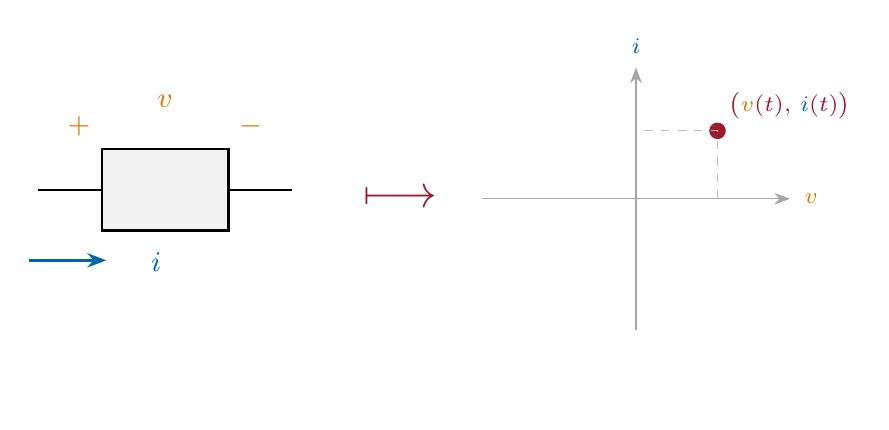
\begin{tikzpicture}[scale=1.15, transform shape]
    \begin{scope}[yshift=0.1cm]
      \draw[thick] (0,0) -- (0.7,0); \draw[thick] (2.1,0) -- (2.8,0);
      \draw[thick, fill=gray!10] (0.7,-0.45) rectangle (2.1,0.45);
      \node[pol] at (0.45,0.7) {$+$}; \node[pol] at (2.35,0.7) {$-$};
      \node[pol] at (1.4,0.98) {$v$};
      \draw[iar] (-0.1,-0.78) -- (0.75,-0.78);
      \node[ccur, font=\small] at (1.3,-0.8) {$i$};
    \end{scope}
    \node[font=\Large, text=metured] at (4.0,0) {$\longmapsto$};
    \begin{scope}[xshift=6.6cm]
      \viaxes{1.7}{1.45}{}
      \fill[metured] (0.9,0.75) circle (2.6pt);
      \node[font=\scriptsize, text=metured, above right=0pt] at (0.9,0.75)
           {$\big(\Vcol{v}(t),\,\Icol{i}(t)\big)$};
      \draw[gray!55, dashed] (0.9,0) -- (0.9,0.75) -- (0,0.75);
    \end{scope}
  \end{tikzpicture}
  \end{center}
  \vfill
  \begin{center}
    As time passes, the point moves.\\
    The element is defined by \alert{which points it is allowed to visit}.
  \end{center}
  \vfill
\end{frame}

%--------------------------------------------------------------
\begin{frame}{The characteristic}
  \vfill
  \begin{center}
    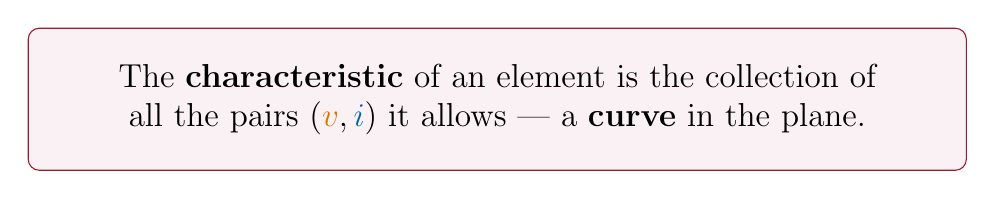
\begin{tikzpicture}
      \node[draw=metured, fill=metured!6, rounded corners=4pt, inner sep=13pt,
            text width=11.0cm, align=center, font=\large]
      {The \textbf{characteristic} of an element is the collection of \alert{all} the
       pairs $(\Vcol{v},\Icol{i})$ it allows --- a \textbf{curve} in the plane.};
    \end{tikzpicture}
  \end{center}
  \vfill
  \begin{columns}[c,onlytextwidth]
    \begin{column}{0.40\textwidth}
      \begin{center}
      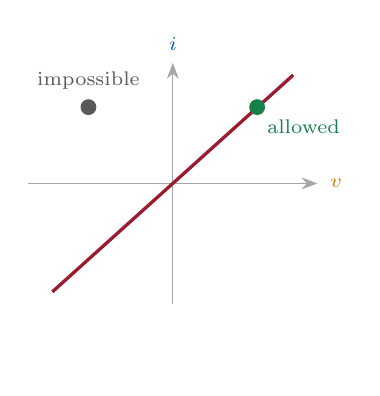
\begin{tikzpicture}[scale=1.02, transform shape]
        \viaxes{1.8}{1.5}{}
        \draw[crv] (-1.5,-1.35) -- (1.5,1.35);
        \fill[cpow, visible on=<2->] (1.05,0.95) circle (2.8pt);
        \node[font=\scriptsize, text=cpow, below right=0pt, visible on=<2->]
             at (1.05,0.92) {allowed};
        \fill[metugray, visible on=<3->] (-1.05,0.95) circle (2.8pt);
        \node[font=\scriptsize, text=metugray, above=2pt, visible on=<3->]
             at (-1.05,0.98) {impossible};
      \end{tikzpicture}
      \end{center}
    \end{column}
    \begin{column}{0.56\textwidth}
      \onslide<2->{The operating point may sit \alert{anywhere on the curve}}
      \onslide<3->{and \alert{nowhere else}.}
      \\[10pt]
      \onslide<4->{Give the element a voltage and the curve tells you the current ---
      and the other way round.}
    \end{column}
  \end{columns}
  \vfill
\end{frame}

%--------------------------------------------------------------
\begin{frame}{Every element is a curve}
  \vfill
  \begin{center}
    {\Huge\color{metured} \emph{which curve?}}
  \end{center}
  \vfill
  \begin{center}
  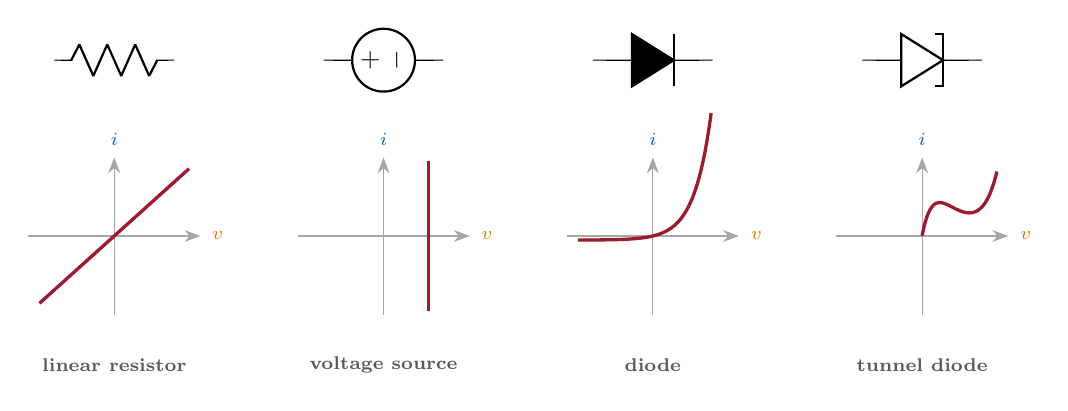
\begin{tikzpicture}[scale=0.95, transform shape]
    \def\W{1.15} \def\H{1.05} \def\S{3.6}
    \begin{scope}
      \draw (-0.8,2.35) to[R] (0.8,2.35);
      \viaxes{\W}{\H}{linear resistor}
      \draw[crv] (-1.0,-0.9) -- (1.0,0.9);
    \end{scope}
    \begin{scope}[xshift=\S cm]
      \draw (-0.8,2.35) to[american voltage source] (0.8,2.35);
      \viaxes{\W}{\H}{voltage source}
      \draw[crv] (0.6,-1.0) -- (0.6,1.0);
    \end{scope}
    \begin{scope}[xshift=2*\S cm]
      \draw (-0.8,2.35) to[full diode] (0.8,2.35);
      \viaxes{\W}{\H}{diode}
      \draw[crv, domain=-1.0:0.78, samples=140, smooth] plot (\x, {0.055*(exp(4.4*\x)-1)});
    \end{scope}
    \begin{scope}[xshift=3*\S cm]
      \draw (-0.8,2.35) to[tunnel diode] (0.8,2.35);
      \viaxes{\W}{\H}{tunnel diode}
      \draw[crv, domain=0:1.0, samples=180, smooth]
           plot (\x, {5.2*\x*exp(-4.4*\x) + 0.8*exp(5.5*(\x-1.0))});
    \end{scope}
  \end{tikzpicture}
  \end{center}
  \vfill
  \begin{center}
    {\large Four devices. Four curves. One plane.}
  \end{center}
  \vfill
\end{frame}

%--------------------------------------------------------------
\begin{frame}{The independent voltage source}
  \vfill
  \begin{center}
  \begin{tikzpicture}[scale=1.0, transform shape]
    \begin{scope}[yshift=-0.1cm]
      \draw (0,0) to[american voltage source, invert] (0,2.0);
      \node[pol] at (0.68,1.42) {$+$}; \node[pol] at (0.68,0.52) {$-$};
      \node[pol] at (1.02,0.97) {$v$};
      \draw[iar] (-0.62,0.62) -- (-0.62,1.32); \node[ccur, font=\small] at (-0.95,0.97) {$i$};
    \end{scope}
    \node[font=\Large, text=metured] at (2.2,0.9) {$\longmapsto$};
    \begin{scope}[xshift=5.0cm, yshift=0.9cm]
      \viaxes{1.6}{1.35}{}
      \draw[crv] (0.8,-1.25) -- (0.8,1.25);
      \node[font=\scriptsize, text=cvolt] at (1.2,-0.9) {$v_s$};
    \end{scope}
    \node[font=\normalsize, anchor=west, text width=4.9cm] at (7.0,0.9)
      {\[ \Vcol{v}(t) = v_s(t) \]
       \vspace{-4pt}
       \begin{center}for \alert{every} $\Icol{i}$\end{center}
       \vspace{2pt}
       \footnotesize A \textbf{vertical line}, which may slide sideways as $t$ runs.};
  \end{tikzpicture}
  \end{center}
  \vfill
\end{frame}

%--------------------------------------------------------------
\begin{frame}{Two symbols, one element}
  \vfill
  \begin{center}
  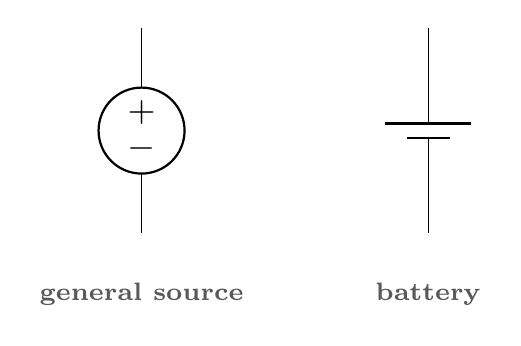
\begin{tikzpicture}[scale=1.3, transform shape]
    \begin{scope}
      \draw (0,0) to[american voltage source, invert] (0,2.0);
      \node[ttl] at (0,-0.6) {general source};
    \end{scope}
    \begin{scope}[xshift=2.8cm]
      \draw (0,0) to[battery1, invert] (0,2.0);
      \node[ttl] at (0,-0.6) {battery};
    \end{scope}
  \end{tikzpicture}
  \end{center}
  \vfill
  \begin{center}
    Both are independent voltage sources; both appear in books, in the lab and in this
    course.\\[6pt]
    The battery symbol hints that the source is \emph{constant}; the circle covers any
    $v_s(t)$.\\[8pt]
    {\large We will use the \alert{circle} from here on.}
  \end{center}
  \vfill
\end{frame}

%--------------------------------------------------------------
\begin{frame}{A source does not decide the other variable}
  \vfill
  \begin{center}
  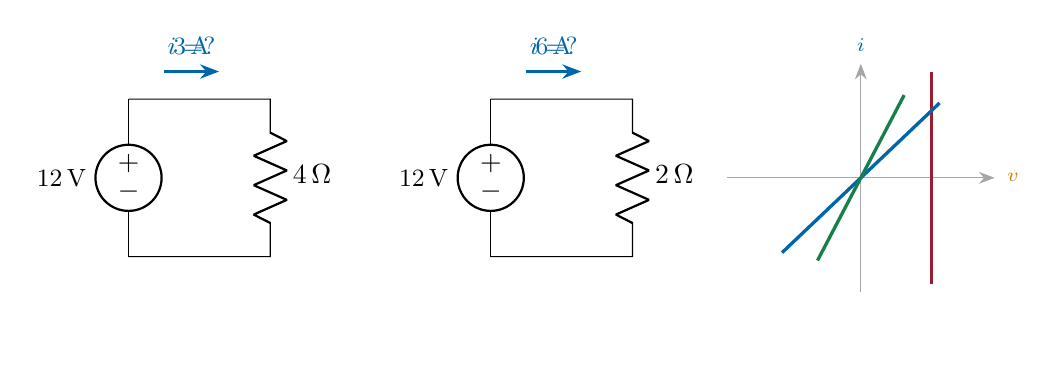
\begin{tikzpicture}[scale=1.0, transform shape]
    \begin{scope}
      \draw (0,0) to[american voltage source, invert] (0,2.0);
      \draw (0,2.0) -- (1.8,2.0) to[R, l=$4\ohm$] (1.8,0) -- (0,0);
      \draw[iar] (0.45,2.35) -- (1.15,2.35);
      \node[ccur, font=\small, visible on=<1>] at (0.8,2.68) {$\Icol{i} = ?$};
      \node[ccur, font=\small, visible on=<2->] at (0.8,2.68) {$3\A$};
      \node[font=\small] at (-0.85,1.0) {$12\V$};
    \end{scope}
    \begin{scope}[xshift=4.6cm]
      \draw (0,0) to[american voltage source, invert] (0,2.0);
      \draw (0,2.0) -- (1.8,2.0) to[R, l=$2\ohm$] (1.8,0) -- (0,0);
      \draw[iar] (0.45,2.35) -- (1.15,2.35);
      \node[ccur, font=\small, visible on=<1>] at (0.8,2.68) {$\Icol{i} = ?$};
      \node[ccur, font=\small, visible on=<2->] at (0.8,2.68) {$6\A$};
      \node[font=\small] at (-0.85,1.0) {$12\V$};
    \end{scope}
    \begin{scope}[xshift=9.3cm, yshift=1.0cm]
      \viaxes{1.7}{1.45}{}
      \draw[crv, visible on=<3->] (0.9,-1.35) -- (0.9,1.35);
      \draw[ccur, very thick, visible on=<3->] (-1.0,-0.95) -- (1.0,0.95);
      \draw[cpow, very thick, visible on=<3->] (-0.55,-1.05) -- (0.55,1.05);
    \end{scope}
  \end{tikzpicture}
  \end{center}
  \vfill
  \begin{center}
    \onslide<3->{The source's line \alert{never moved}. The other element's line did.\\[4pt]}
    \onslide<4->{Which current flows is settled by KCL, KVL and the rest of the circuit ---
    never by the source alone.}
  \end{center}
  \vfill
\end{frame}

%--------------------------------------------------------------
\begin{frame}{$v_s(t)$ can be any function you like}
  \vfill
  \begin{center}
  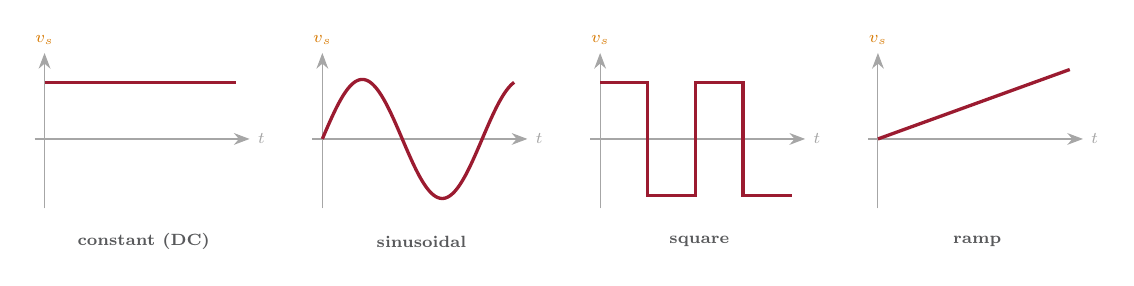
\begin{tikzpicture}[scale=0.84, transform shape]
   \foreach \dx/\ttlx in {0/{constant (DC)}, 4.2/{sinusoidal}, 8.4/{square}, 12.6/{ramp}}{
     \begin{scope}[xshift=\dx cm]
       \draw[vax] (-0.15,0) -- (3.1,0) node[right, font=\scriptsize] {$t$};
       \draw[vax] (0,-1.05) -- (0,1.3) node[above, font=\scriptsize, text=cvolt] {$v_s$};
       \node[ttl] at (1.5,-1.55) {\ttlx};
     \end{scope}}
   \draw[crv] (0,0.85) -- (2.9,0.85);
   \begin{scope}[xshift=4.2cm]
     \draw[crv, domain=0:2.9, samples=120, smooth] plot (\x, {0.9*sin(deg(2.6*\x))});
   \end{scope}
   \begin{scope}[xshift=8.4cm]
     \draw[crv] (0,0.85)--(0.72,0.85)--(0.72,-0.85)--(1.44,-0.85)--(1.44,0.85)
                --(2.16,0.85)--(2.16,-0.85)--(2.9,-0.85);
   \end{scope}
   \begin{scope}[xshift=12.6cm]
     \draw[crv] (0,0) -- (2.9,1.05);
   \end{scope}
  \end{tikzpicture}
  \end{center}
  \vfill
  \begin{center}
    The characteristic stays a vertical line throughout --- it just slides.
  \end{center}
  \vfill
\end{frame}

%--------------------------------------------------------------
\begin{frame}{The independent current source}
  \vfill
  \begin{center}
  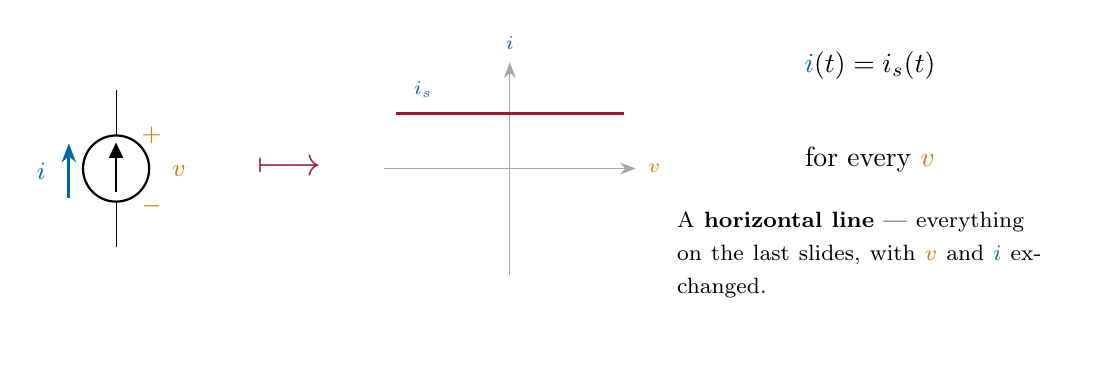
\begin{tikzpicture}[scale=1.0, transform shape]
    \begin{scope}[yshift=-0.1cm]
      \draw (0,0) to[american current source] (0,2.0);
      \node[pol] at (0.45,1.42) {$+$}; \node[pol] at (0.45,0.52) {$-$};
      \node[pol] at (0.8,0.97) {$v$};
      \draw[iar] (-0.6,0.62) -- (-0.6,1.32); \node[ccur, font=\small] at (-0.95,0.97) {$i$};
    \end{scope}
    \node[font=\Large, text=metured] at (2.2,0.9) {$\longmapsto$};
    \begin{scope}[xshift=5.0cm, yshift=0.9cm]
      \viaxes{1.6}{1.35}{}
      \draw[crv] (-1.45,0.7) -- (1.45,0.7);
      \node[font=\scriptsize, text=ccur] at (-1.1,1.0) {$i_s$};
    \end{scope}
    \node[font=\normalsize, anchor=west, text width=4.9cm] at (7.0,0.9)
      {\[ \Icol{i}(t) = i_s(t) \]
       \vspace{-4pt}
       \begin{center}for \alert{every} $\Vcol{v}$\end{center}
       \vspace{2pt}
       \footnotesize A \textbf{horizontal line} --- everything on the last slides, with
       $\Vcol{v}$ and $\Icol{i}$ exchanged.};
  \end{tikzpicture}
  \end{center}
  \vfill
  \begin{center}\small\color{metugray}
    $2\A$ into $4\ohm$ makes $8\V$; into $100\ohm$ it makes $200\V$; into an open circuit
    the ideal model demands infinity --- which is the model warning you that a real source
    has a limit.
  \end{center}
  \vfill
\end{frame}

%--------------------------------------------------------------
\begin{frame}{Two familiar elements, renamed}
  \vfill
  \begin{center}
  \begin{tikzpicture}[scale=0.98, transform shape]
    \begin{scope}
      \draw[thick] (0,0) -- (2.2,0);
      \fill[metured] (0,0) circle (2.2pt); \fill[metured] (2.2,0) circle (2.2pt);
      \node[ttl] at (1.1,-0.75) {short circuit};
    \end{scope}
    \begin{scope}[xshift=3.7cm, yshift=0.1cm]
      \viaxes{1.3}{1.15}{$v_s = 0$}
      \draw[crv] (0,-1.1) -- (0,1.1);
    \end{scope}
    \begin{scope}[xshift=7.2cm]
      \draw[thick] (0,0) -- (0.8,0); \draw[thick] (1.4,0) -- (2.2,0);
      \fill[metured] (0,0) circle (2.2pt); \fill[metured] (2.2,0) circle (2.2pt);
      \node[ttl] at (1.1,-0.75) {open circuit};
    \end{scope}
    \begin{scope}[xshift=10.9cm, yshift=0.1cm]
      \viaxes{1.3}{1.15}{$i_s = 0$}
      \draw[crv] (-1.25,0) -- (1.25,0);
    \end{scope}
  \end{tikzpicture}
  \end{center}
  \vfill
  \begin{center}
    A short circuit \emph{is} a voltage source of zero volts.\\
    An open circuit \emph{is} a current source of zero amperes.
  \end{center}
  \vfill
\end{frame}

%--------------------------------------------------------------
\begin{frame}{Which quadrant is the element in?}
  \vfill
  \begin{center}
  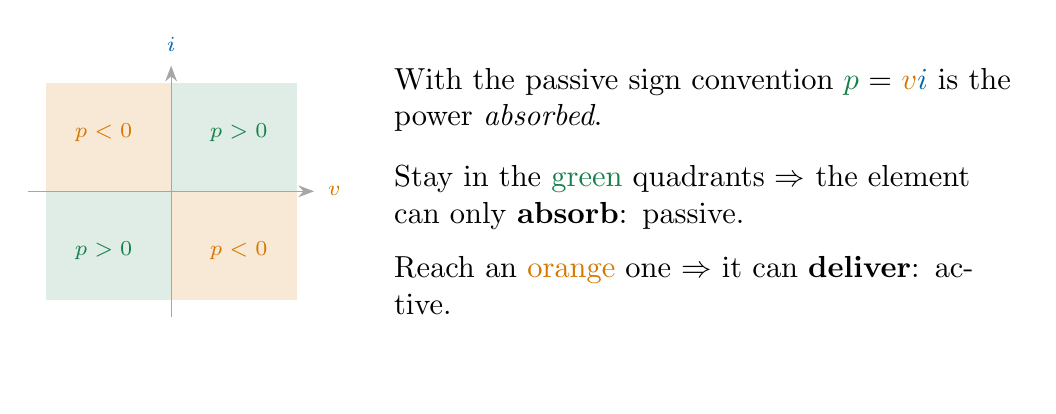
\begin{tikzpicture}[scale=1.1, transform shape]
    \fill[cpow!14] (0,0) rectangle (1.45,1.25);
    \fill[cpow!14] (0,0) rectangle (-1.45,-1.25);
    \fill[cvolt!16] (0,0) rectangle (-1.45,1.25);
    \fill[cvolt!16] (0,0) rectangle (1.45,-1.25);
    \viaxes{1.65}{1.45}{}
    \node[font=\scriptsize, text=cpow] at (0.78,0.68) {$p > 0$};
    \node[font=\scriptsize, text=cpow] at (-0.78,-0.68) {$p > 0$};
    \node[font=\scriptsize, text=cvolt] at (-0.78,0.68) {$p < 0$};
    \node[font=\scriptsize, text=cvolt] at (0.78,-0.68) {$p < 0$};
    \node[font=\normalsize, anchor=west, text width=7.2cm] at (2.45,0)
      {With the passive sign convention $\Pcol{p} = \Vcol{v}\Icol{i}$ is the power
       \emph{absorbed}.\\[8pt]
       Stay in the \textcolor{cpow}{green} quadrants $\Rightarrow$ the element can only
       \textbf{absorb}: \alert{passive}.\\[6pt]
       Reach an \textcolor{cvolt}{orange} one $\Rightarrow$ it can \textbf{deliver}:
       \alert{active}.};
  \end{tikzpicture}
  \end{center}
  \vfill
\end{frame}

%--------------------------------------------------------------
\begin{frame}{Every independent source is active}
  \vfill
  \begin{center}
  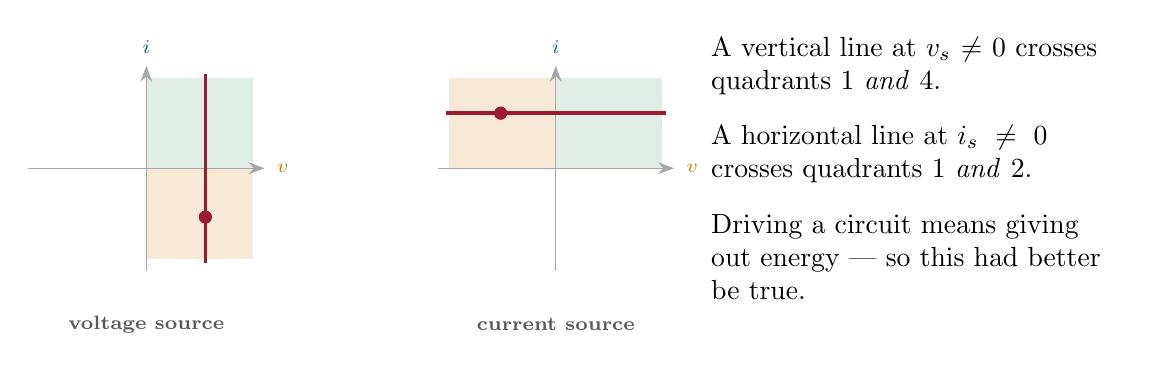
\begin{tikzpicture}[scale=1.0, transform shape]
    \begin{scope}
      \fill[cpow!14] (0,0) rectangle (1.35,1.15);
      \fill[cvolt!16] (0,0) rectangle (1.35,-1.15);
      \viaxes{1.5}{1.3}{voltage source}
      \draw[crv] (0.75,-1.2) -- (0.75,1.2);
      \fill[metured] (0.75,-0.62) circle (2.4pt);
    \end{scope}
    \begin{scope}[xshift=5.2cm]
      \fill[cpow!14] (0,0) rectangle (1.35,1.15);
      \fill[cvolt!16] (0,0) rectangle (-1.35,1.15);
      \viaxes{1.5}{1.3}{current source}
      \draw[crv] (-1.4,0.7) -- (1.4,0.7);
      \fill[metured] (-0.7,0.7) circle (2.4pt);
    \end{scope}
    \node[font=\normalsize, anchor=west, text width=5.1cm] at (7.05,0)
      {A vertical line at $v_s \neq 0$ crosses quadrants 1 \emph{and} 4.\\[8pt]
       A horizontal line at $i_s \neq 0$ crosses quadrants 1 \emph{and} 2.\\[8pt]
       Driving a circuit means giving out energy --- so this had better be true.};
  \end{tikzpicture}
  \end{center}
  \vfill
\end{frame}

%--------------------------------------------------------------
\begin{frame}{What is a resistor?}
  \vfill
  \begin{center}
    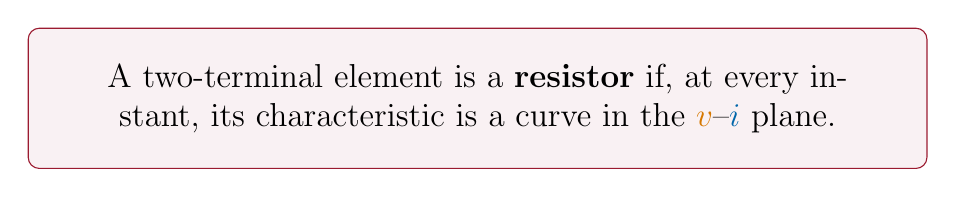
\begin{tikzpicture}
      \node[draw=metured, fill=metured!6, rounded corners=4pt, inner sep=13pt,
            text width=10.5cm, align=center, font=\large]
      {A two-terminal element is a \textbf{resistor} if, at every instant, its
       characteristic is a \alert{curve} in the $\Vcol{v}$--$\Icol{i}$ plane.};
    \end{tikzpicture}
  \end{center}
  \vfill
  \begin{center}
    Nothing about straight lines. Nothing about Ohm's law. Nothing about $R$.\\[8pt]
    {\large The relation between $\Vcol{v}$ and $\Icol{i}$ is \alert{purely algebraic}
     --- no derivatives, \alert{no memory}.}
  \end{center}
  \vfill
\end{frame}

%--------------------------------------------------------------
\begin{frame}{So the family is large}
  \vfill
  \begin{columns}[T,onlytextwidth]
    \begin{column}{0.48\textwidth}
      \begin{block}{Resistors}
        \small
        diodes, tunnel diodes, light bulbs, thermistors\\[4pt]
        short circuits, open circuits\\[4pt]
        \alert{independent sources} --- a straight line, just not through the origin
      \end{block}
    \end{column}
    \begin{column}{0.48\textwidth}
      \begin{block}{Not resistors}
        \small
        \begin{center}
          $\Icol{i} = C\,\dfrac{d\Vcol{v}}{dt}$ \qquad $\Vcol{v} = L\,\dfrac{d\Icol{i}}{dt}$
        \end{center}
        \vspace{2pt}
        the same $\Vcol{v}$ allows \emph{any} $\Icol{i}$, depending on how $\Vcol{v}$ is
        changing --- so it is not a curve
      \end{block}
    \end{column}
  \end{columns}
  \vfill
  \begin{center}
    Yes --- that makes a \alert{battery} a resistor.\\[4pt]
    The word describes the \emph{shape of the relation}, not dissipation.
    Read it as \alert{``memoryless element''}.
  \end{center}
  \vfill
\end{frame}

%--------------------------------------------------------------
\begin{frame}{A gallery of resistors}
  \vfill
  \begin{center}
  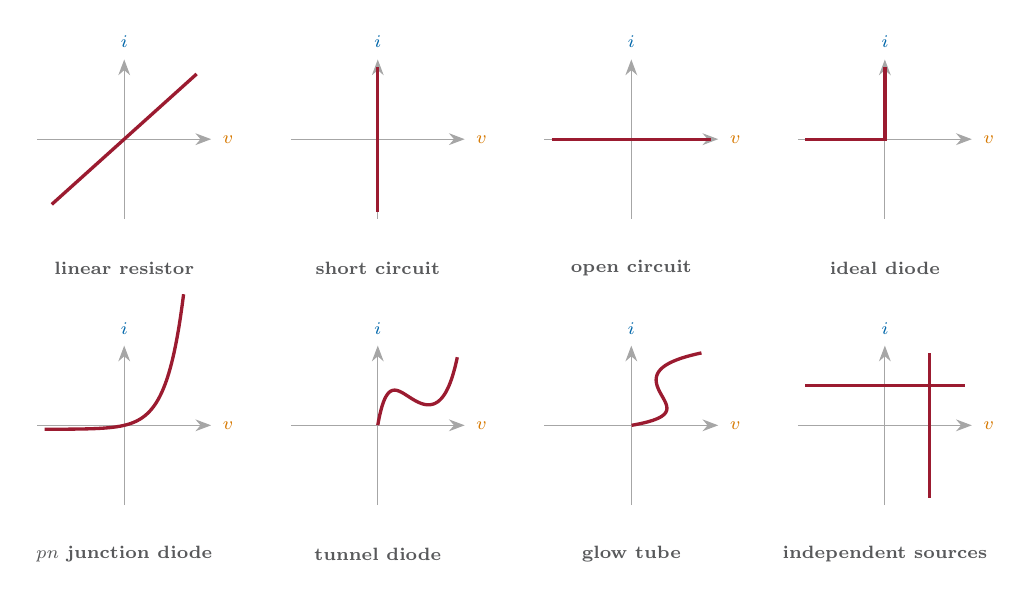
\begin{tikzpicture}[scale=0.92, transform shape]
    \def\W{1.2} \def\H{1.1} \def\S{3.5}
    \begin{scope}
      \viaxes{\W}{\H}{linear resistor}
      \draw[crv] (-1.0,-0.9) -- (1.0,0.9);
    \end{scope}
    \begin{scope}[xshift=\S cm]
      \viaxes{\W}{\H}{short circuit}
      \draw[crv] (0,-1.0) -- (0,1.0);
    \end{scope}
    \begin{scope}[xshift=2*\S cm]
      \viaxes{\W}{\H}{open circuit}
      \draw[crv] (-1.1,0) -- (1.1,0);
    \end{scope}
    \begin{scope}[xshift=3*\S cm]
      \viaxes{\W}{\H}{ideal diode}
      \draw[crv] (-1.1,0) -- (0,0) -- (0,1.0);
    \end{scope}
    \begin{scope}[yshift=-3.95cm]
      \viaxes{\W}{\H}{$pn$ junction diode}
      \draw[crv, domain=-1.1:0.82, samples=140, smooth] plot (\x, {0.055*(exp(4.3*\x)-1)});
    \end{scope}
    \begin{scope}[xshift=\S cm, yshift=-3.95cm]
      \viaxes{\W}{\H}{tunnel diode}
      \draw[crv, domain=0:1.1, samples=180, smooth]
           plot (\x, {5.72*\x*exp(-4.4*\x) + 0.9*exp(5.5*(\x-1.1))});
    \end{scope}
    \begin{scope}[xshift=2*\S cm, yshift=-3.95cm]
      \viaxes{\W}{\H}{glow tube}
      \draw[crv, domain=0:1.0, samples=180, smooth]
           plot ({5.72*\x*exp(-4.4*\x) + 0.9*exp(5.5*(\x-1.0))}, \x);
    \end{scope}
    \begin{scope}[xshift=3*\S cm, yshift=-3.95cm]
      \viaxes{\W}{\H}{independent sources}
      \draw[crv] (0.62,-1.0) -- (0.62,1.0);
      \draw[crv] (-1.1,0.55) -- (1.1,0.55);
    \end{scope}
  \end{tikzpicture}
  \end{center}
  \vfill
\end{frame}

%--------------------------------------------------------------
\begin{frame}{Linear}
  \vfill
  \begin{center}
    {\large A straight line \alert{through the origin}.}
  \end{center}
  \vfill
  \begin{center}
  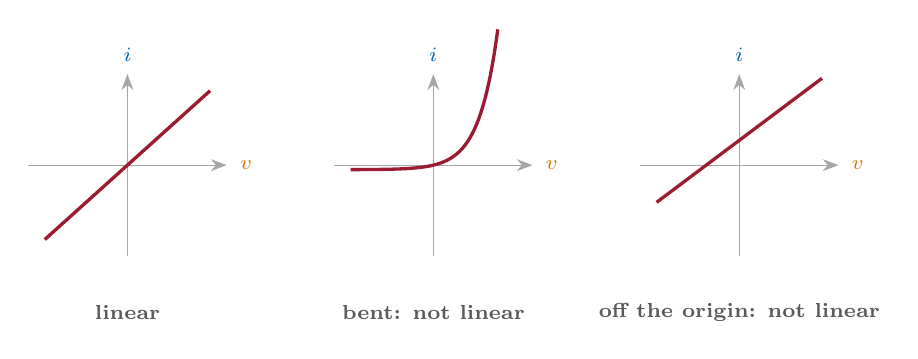
\begin{tikzpicture}[scale=1.05, transform shape]
    \def\W{1.2} \def\H{1.1} \def\S{3.7}
    \begin{scope}
      \viaxes{\W}{\H}{linear}
      \draw[crv] (-1.0,-0.9) -- (1.0,0.9);
    \end{scope}
    \begin{scope}[xshift=\S cm]
      \viaxes{\W}{\H}{bent: not linear}
      \draw[crv, domain=-1.0:0.78, samples=140, smooth] plot (\x, {0.055*(exp(4.4*\x)-1)});
    \end{scope}
    \begin{scope}[xshift=2*\S cm]
      \viaxes{\W}{\H}{off the origin: not linear}
      \draw[crv] (-1.0,-0.45) -- (1.0,1.05);
    \end{scope}
  \end{tikzpicture}
  \end{center}
  \vfill
  \begin{center}
    A battery is perfectly straight and \alert{not} a linear element.
  \end{center}
  \vfill
\end{frame}

%--------------------------------------------------------------
\begin{frame}{Bilateral}
  \vfill
  \begin{center}
    {\large Symmetric about the origin: if $(\Vcol{v},\Icol{i})$ is on the curve,
     so is $(-\Vcol{v},-\Icol{i})$.}
  \end{center}
  \vfill
  \begin{center}
  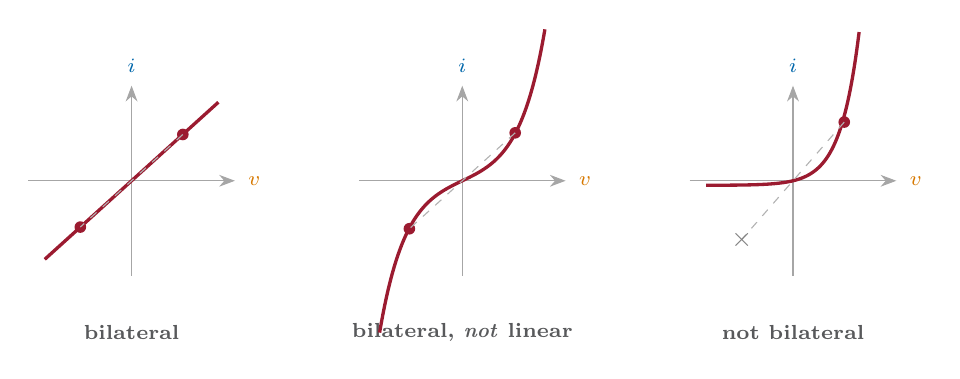
\begin{tikzpicture}[scale=1.05, transform shape]
    \def\S{4.0}
    \begin{scope}
      \viaxes{1.25}{1.15}{bilateral}
      \draw[crv] (-1.05,-0.95) -- (1.05,0.95);
      \fill[metured] (0.62,0.56) circle (2.0pt); \fill[metured] (-0.62,-0.56) circle (2.0pt);
      \draw[gray!60, dashed] (0.62,0.56) -- (-0.62,-0.56);
    \end{scope}
    \begin{scope}[xshift=\S cm]
      \viaxes{1.25}{1.15}{bilateral, \emph{not} linear}
      \draw[crv, domain=-1.0:1.0, samples=160, smooth]
           plot (\x, {0.075*(exp(3.2*\x)-exp(-3.2*\x))});
      \fill[metured] (0.64,0.58) circle (2.0pt); \fill[metured] (-0.64,-0.58) circle (2.0pt);
      \draw[gray!60, dashed] (0.64,0.58) -- (-0.64,-0.58);
    \end{scope}
    \begin{scope}[xshift=2*\S cm]
      \viaxes{1.25}{1.15}{not bilateral}
      \draw[crv, domain=-1.05:0.8, samples=140, smooth] plot (\x, {0.055*(exp(4.4*\x)-1)});
      \fill[metured] (0.62,0.71) circle (2.0pt);
      \draw[gray!60, dashed] (0.62,0.71) -- (-0.62,-0.71);
      \node[gray, font=\small] at (-0.62,-0.71) {$\times$};
    \end{scope}
  \end{tikzpicture}
  \end{center}
  \vfill
  \begin{center}
    Turn the element round --- does anything change?\\[6pt]
    The middle one is two diodes back to back: \alert{bent, yet symmetric}.
    Every linear element is bilateral; not the reverse.
  \end{center}
  \vfill
\end{frame}

%--------------------------------------------------------------
\begin{frame}{Voltage-controlled or current-controlled?}
  \vfill
  \begin{center}
    {\large $\Icol{i} = f(\Vcol{v})$ \quad or \quad $\Vcol{v} = g(\Icol{i})$
     \quad --- single-valued which way round?}
  \end{center}
  \vfill
  \begin{center}
  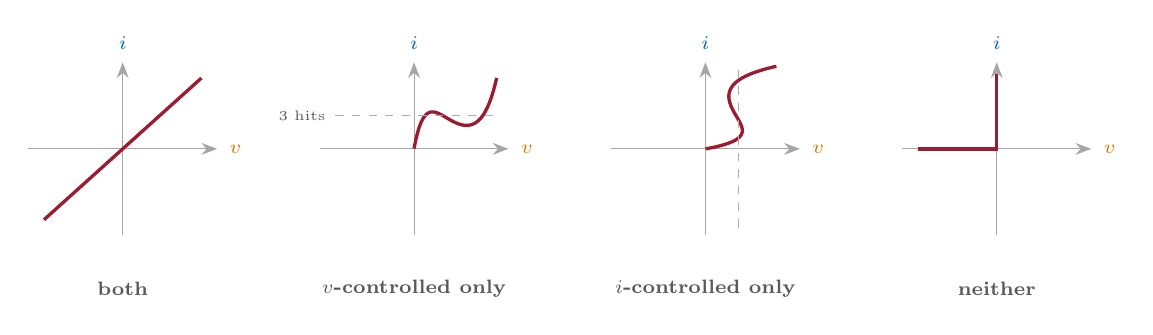
\begin{tikzpicture}[scale=1.0, transform shape]
    \def\W{1.2} \def\H{1.1} \def\S{3.7}
    \begin{scope}
      \viaxes{\W}{\H}{both}
      \draw[crv] (-1.0,-0.9) -- (1.0,0.9);
    \end{scope}
    \begin{scope}[xshift=\S cm]
      \viaxes{\W}{\H}{$v$-controlled only}
      \draw[crv, domain=0:1.05, samples=180, smooth]
           plot (\x, {5.5*\x*exp(-4.4*\x) + 0.85*exp(5.5*(\x-1.05))});
      \draw[gray!65, dashed] (-1.0,0.42) -- (1.05,0.42);
      \node[font=\tiny, text=metugray, left] at (-1.0,0.42) {3 hits};
    \end{scope}
    \begin{scope}[xshift=2*\S cm]
      \viaxes{\W}{\H}{$i$-controlled only}
      \draw[crv, domain=0:1.05, samples=180, smooth]
           plot ({5.5*\x*exp(-4.4*\x) + 0.85*exp(5.5*(\x-1.05))}, \x);
      \draw[gray!65, dashed] (0.42,-1.0) -- (0.42,1.05);
    \end{scope}
    \begin{scope}[xshift=3*\S cm]
      \viaxes{\W}{\H}{neither}
      \draw[crv] (-1.0,0) -- (0,0) -- (0,0.95);
    \end{scope}
  \end{tikzpicture}
  \end{center}
  \vfill
  \begin{center}\small
    The ideal diode fails both: at $\Vcol{v} = 0$ any positive current is allowed,
    and at $\Icol{i} = 0$ any negative voltage is.
  \end{center}
  \vfill
\end{frame}

%--------------------------------------------------------------
\begin{frame}{Time-invariant}
  \vfill
  \begin{center}
    {\large Is it \alert{the same curve} at every instant?}
  \end{center}
  \vfill
  \begin{center}
  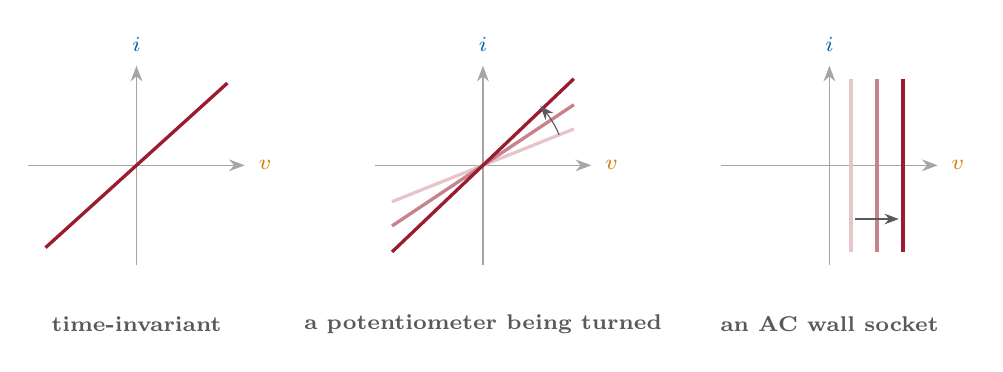
\begin{tikzpicture}[scale=1.1, transform shape]
    \def\W{1.25} \def\H{1.15} \def\S{4.0}
    \begin{scope}
      \viaxes{\W}{\H}{time-invariant}
      \draw[crv] (-1.05,-0.95) -- (1.05,0.95);
    \end{scope}
    \begin{scope}[xshift=\S cm]
      \viaxes{\W}{\H}{a potentiometer being turned}
      \draw[metured!25, very thick] (-1.05,-0.42) -- (1.05,0.42);
      \draw[metured!55, very thick] (-1.05,-0.7) -- (1.05,0.7);
      \draw[crv] (-1.05,-1.0) -- (1.05,1.0);
      \draw[-{Stealth[length=1.8mm]}, metugray] (0.88,0.35) arc (22:44:1.05);
    \end{scope}
    \begin{scope}[xshift=2*\S cm]
      \viaxes{\W}{\H}{an AC wall socket}
      \draw[metured!25, very thick] (0.25,-1.0) -- (0.25,1.0);
      \draw[metured!55, very thick] (0.55,-1.0) -- (0.55,1.0);
      \draw[crv] (0.85,-1.0) -- (0.85,1.0);
      \draw[-{Stealth[length=1.8mm]}, metugray] (0.3,-0.62) -- (0.8,-0.62);
    \end{scope}
  \end{tikzpicture}
  \end{center}
  \vfill
  \begin{center}
    Still a curve at every instant --- but a \alert{different} one.
  \end{center}
  \vfill
\end{frame}

%--------------------------------------------------------------
\begin{frame}{The gallery, characterized}
  \vfill
  \begin{center}
  \footnotesize
  \renewcommand{\arraystretch}{1.18}
  \begin{tabular}{@{}l c c c c c c@{}}
    \toprule
    \textbf{Element} & linear & bilateral & passive & $v$-contr. & $i$-contr. & time-inv.\\
    \midrule
    linear resistor, $R>0$        & yes & yes & yes & yes & yes & yes\\
    linear resistor, $R<0$        & yes & yes & \alert{no}  & yes & yes & yes\\
    short circuit                 & yes & yes & yes & \alert{no}  & yes & yes\\
    open circuit                  & yes & yes & yes & yes & \alert{no}  & yes\\
    ideal diode                   & \alert{no} & \alert{no} & yes & \alert{no} & \alert{no} & yes\\
    $pn$ junction diode           & \alert{no} & \alert{no} & yes & yes & yes & yes\\
    tunnel diode                  & \alert{no} & \alert{no} & yes & yes & \alert{no} & yes\\
    glow tube                     & \alert{no} & \alert{no} & yes & \alert{no} & yes & yes\\
    DC voltage source, $v_s\neq0$ & \alert{no} & \alert{no} & \alert{no} & \alert{no} & yes & yes\\
    DC current source, $i_s\neq0$ & \alert{no} & \alert{no} & \alert{no} & yes & \alert{no} & yes\\
    AC voltage source             & \alert{no} & \alert{no} & \alert{no} & \alert{no} & yes & \alert{no}\\
    \bottomrule
  \end{tabular}
  \end{center}
  \vfill
\end{frame}

%--------------------------------------------------------------
\begin{frame}{Three rows, read off the picture}
  \vfill
  \begin{center}
  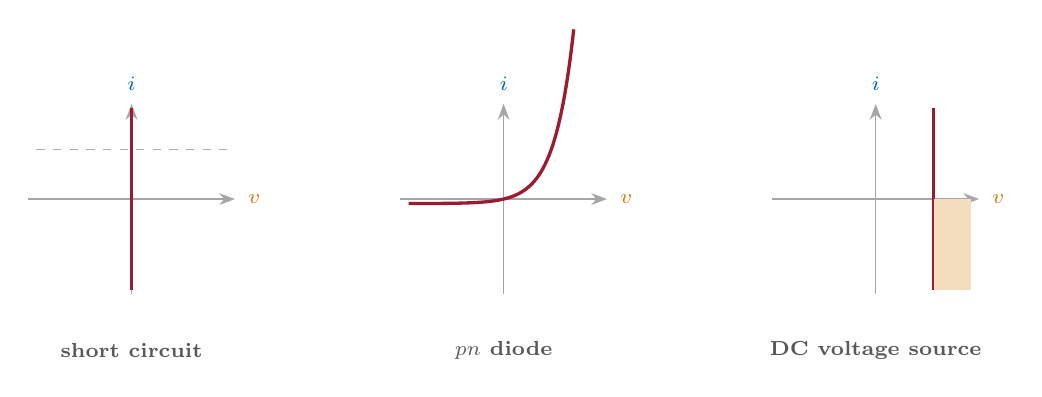
\begin{tikzpicture}[scale=1.05, transform shape]
    \begin{scope}
      \viaxes{1.25}{1.15}{short circuit}
      \draw[crv] (0,-1.1) -- (0,1.1);
      \draw[gray!65, dashed, visible on=<2->] (-1.15,0.6) -- (1.15,0.6);
    \end{scope}
    \begin{scope}[xshift=4.5cm]
      \viaxes{1.25}{1.15}{$pn$ diode}
      \draw[crv, domain=-1.15:0.85, samples=140, smooth] plot (\x, {0.055*(exp(4.3*\x)-1)});
    \end{scope}
    \begin{scope}[xshift=9.0cm]
      \viaxes{1.25}{1.15}{DC voltage source}
      \draw[crv] (0.7,-1.1) -- (0.7,1.1);
      \fill[cvolt!25, visible on=<4->] (0.7,0) rectangle (1.15,-1.1);
    \end{scope}
  \end{tikzpicture}
  \end{center}
  \vfill
  \begin{columns}[T,onlytextwidth]
    \begin{column}{0.31\textwidth}
      \onslide<2->{\small At $\Vcol{v}=0$ \emph{any} current is allowed $\Rightarrow$ not
      $v$-controlled. But $\Vcol{v}=g(\Icol{i})=0$ always $\Rightarrow$ $i$-controlled.}
    \end{column}
    \begin{column}{0.31\textwidth}
      \onslide<3->{\small Single-valued and increasing both ways $\Rightarrow$ controlled by
      either. Stays in quadrants 1 and 3 $\Rightarrow$ passive.}
    \end{column}
    \begin{column}{0.31\textwidth}
      \onslide<4->{\small Misses the origin $\Rightarrow$ not linear. Reaches quadrant 4
      $\Rightarrow$ active. Any $\Icol{i}$ at $\Vcol{v}=v_s$ $\Rightarrow$ not
      $v$-controlled.}
    \end{column}
  \end{columns}
  \vfill
\end{frame}

%--------------------------------------------------------------
\begin{frame}{The LTI resistor}
  \vfill
  \begin{center}
    {\large Take two of those five words: \alert{linear} and \alert{time-invariant}.}\\[6pt]
    A straight line through the origin, and it never moves. Only the slope is left.
  \end{center}
  \vfill
  \begin{center}
  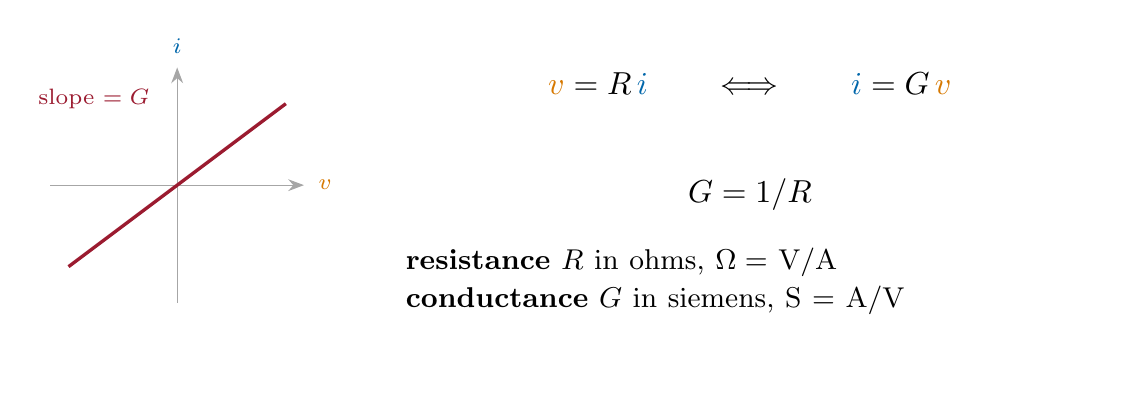
\begin{tikzpicture}[scale=1.15, transform shape]
    \viaxes{1.4}{1.3}{}
    \draw[crv] (-1.2,-0.9) -- (1.2,0.9);
    \node[font=\scriptsize, text=metured] at (-0.92,0.95) {slope $=G$};
    \node[font=\normalsize, anchor=west, text width=7.6cm] at (2.4,0)
      {\[ \Vcol{v} = R\,\Icol{i} \qquad\Longleftrightarrow\qquad \Icol{i} = G\,\Vcol{v} \]
       \vspace{-4pt}
       \begin{center}$G = 1/R$\end{center}
       \vspace{2pt}
       \small \textbf{resistance} $R$ in ohms, $\Omega = $ V/A\\
       \textbf{conductance} $G$ in siemens, S $=$ A/V};
  \end{tikzpicture}
  \end{center}
  \vfill
\end{frame}

%--------------------------------------------------------------
\begin{frame}{Turn the line and sweep $R$ from $\infty$ to $0$}
  \vfill
  \begin{center}
  \begin{tikzpicture}[scale=1.1, transform shape]
    \def\W{1.4} \def\H{1.3} \def\S{4.3}
    \begin{scope}
      \viaxes{\W}{\H}{$R = \infty$: open circuit}
      \draw[crv] (-1.3,0) -- (1.3,0);
      \node[font=\scriptsize, text=metugray] at (0.75,-1.0) {$G = 0$};
    \end{scope}
    \begin{scope}[xshift=\S cm]
      \viaxes{\W}{\H}{$0 < R < \infty$}
      \draw[crv] (-1.2,-0.9) -- (1.2,0.9);
    \end{scope}
    \begin{scope}[xshift=2*\S cm]
      \viaxes{\W}{\H}{$R = 0$: short circuit}
      \draw[crv] (0,-1.25) -- (0,1.25);
      \node[font=\scriptsize, text=metugray] at (0.75,-1.0) {$G = \infty$};
    \end{scope}
  \end{tikzpicture}
  \end{center}
  \vfill
  \begin{center}
    A short circuit \alert{fixes the voltage} at zero and lets any current through.\\
    An open circuit \alert{fixes the current} at zero and allows any voltage.
  \end{center}
  \vfill
\end{frame}

%--------------------------------------------------------------
\begin{frame}{$G = 1/R$ --- except at the two ends}
  \vfill
  \begin{center}
  \begin{tabular}{@{}l c c l@{}}
    \toprule
     & $R$ & $G$ & \textbf{characteristic}\\
    \midrule
    short circuit & $0$      & $\infty$ & the $\Icol{i}$-axis, \ $\Vcol{v} = 0$\\
    open circuit  & $\infty$ & $0$      & the $\Vcol{v}$-axis, \ $\Icol{i} = 0$\\
    \bottomrule
  \end{tabular}
  \end{center}
  \vfill
  \begin{center}
    At each end only \alert{one} of the pair is a usable number.\\[6pt]
    {\small Same fact as Lecture 3: a short is current-controlled but not
     voltage-controlled, and an open circuit the other way round.}
  \end{center}
  \vfill
\end{frame}

%--------------------------------------------------------------
\begin{frame}{Power in an LTI resistor}
  \vfill
  \begin{center}
    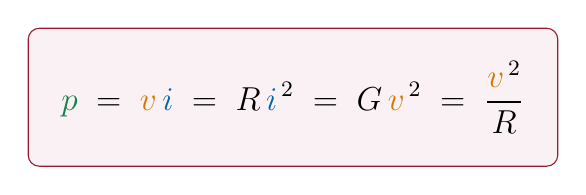
\begin{tikzpicture}
      \node[draw=metured, fill=metured!6, rounded corners=4pt, inner sep=12pt]
      {\large $\displaystyle \Pcol{p} \;=\; \Vcol{v}\,\Icol{i}
        \;=\; R\,\Icol{i}^{\,2} \;=\; G\,\Vcol{v}^{\,2}
        \;=\; \frac{\Vcol{v}^{\,2}}{R}$};
    \end{tikzpicture}
  \end{center}
  \vfill
  \begin{center}
  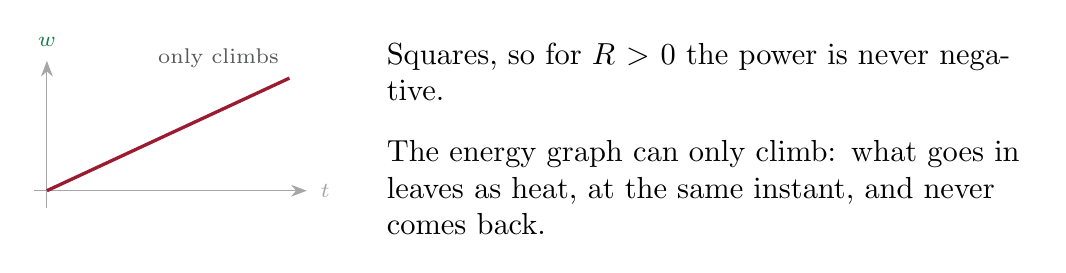
\begin{tikzpicture}[scale=1.1, transform shape]
    \taxes{3.0}{0.2}{1.5}{\Pcol{$w$}}
    \draw[crv] (0,0) -- (2.8,1.3);
    \node[font=\scriptsize, text=metugray, above left] at (2.8,1.3) {only climbs};
    \node[font=\normalsize, anchor=west, text width=7.4cm] at (3.8,0.6)
      {Squares, so for $R>0$ the power is \alert{never negative}.\\[8pt]
       The energy graph can only climb: what goes in leaves as \alert{heat}, at the
       same instant, and never comes back.};
  \end{tikzpicture}
  \end{center}
  \vfill
\end{frame}

%--------------------------------------------------------------
\begin{frame}{Example: a resistor as a heater}
  \vfill
  \begin{columns}[c,onlytextwidth]
    \begin{column}{0.36\textwidth}
      \begin{center}
      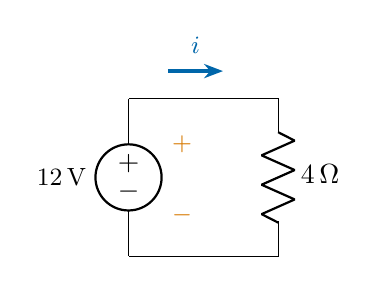
\begin{tikzpicture}[scale=1.0, transform shape]
        \draw (0,0) to[american voltage source, invert] (0,2.0);
        \draw (0,2.0) -- (1.9,2.0) to[R, l=$4\ohm$] (1.9,0) -- (0,0);
        \node[pol] at (0.68,1.42) {$+$}; \node[pol] at (0.68,0.52) {$-$};
        \node[font=\small] at (-0.85,1.0) {$12\V$};
        \draw[iar] (0.5,2.35) -- (1.2,2.35);
        \node[ccur, font=\small] at (0.85,2.68) {$i$};
      \end{tikzpicture}
      \end{center}
    \end{column}
    \begin{column}{0.60\textwidth}
      \[ \Icol{i} = 3\A \]
      \[ \Pcol{p} = 12 \times 3 = 4(3)^2 = 36\W \]
      \[ \Pcol{w}\big|_{10\,\text{min}} = 36 \times 600 = 21.6\uni{kJ} \]
      \vspace{2pt}
      \begin{center}\small
        All of it heat --- which is why a resistor carries a \alert{power rating} as well
        as a resistance.
      \end{center}
    \end{column}
  \end{columns}
  \vfill
\end{frame}

%--------------------------------------------------------------
\begin{frame}{Example: a diode, a source and a resistor}
  \vfill
  \begin{columns}[c,onlytextwidth]
    \begin{column}{0.40\textwidth}
      \begin{center}
      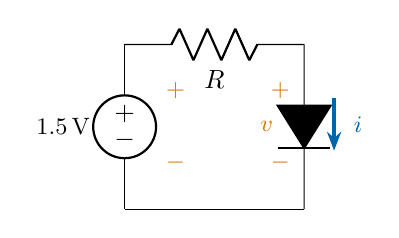
\begin{tikzpicture}[scale=0.95, transform shape]
        \draw (0,0) to[american voltage source, invert] (0,2.2);
        \draw (0,2.2) to[R, l_=$R$] (2.4,2.2);
        \draw (2.4,2.2) to[full diode] (2.4,0);
        \draw (2.4,0) -- (0,0);
        \node[pol] at (0.68,1.58) {$+$}; \node[pol] at (0.68,0.62) {$-$};
        \node[font=\small] at (-0.82,1.1) {$1.5\V$};
        \node[pol] at (2.08,1.58) {$+$}; \node[pol] at (2.08,0.62) {$-$};
        \node[pol] at (1.9,1.1) {$v$};
        \draw[iar] (2.8,1.48) -- (2.8,0.78); \node[ccur, font=\small] at (3.12,1.13) {$i$};
      \end{tikzpicture}
      \end{center}
      \onslide<1>{\begin{center}\large\color{metured}$\Vcol{v} = ?$ \quad $\Icol{i} = ?$\end{center}}
      \onslide<2->{\[ \Icol{i} = \frac{1.5 - \Vcol{v}}{R} \]}
    \end{column}
    \begin{column}{0.58\textwidth}
      \begin{center}
      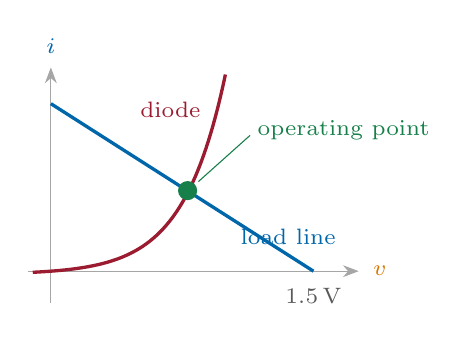
\begin{tikzpicture}[scale=1.15, transform shape]
        \draw[vax] (-0.25,0) -- (3.4,0) node[right=1pt, font=\scriptsize, text=cvolt] {$v$};
        \draw[vax] (0,-0.35) -- (0,2.25) node[above=1pt, font=\scriptsize, text=ccur] {$i$};
        \draw[crv, domain=-0.2:1.93, samples=170, smooth, visible on=<2->] plot (\x, {0.035*(exp(2.15*\x)-1)});
        \node[font=\scriptsize, text=metured, visible on=<2->] at (1.32,1.78) {diode};
        \draw[ccur, very thick, visible on=<3->] (0,1.85) -- (2.9,0);
        \node[font=\scriptsize, text=ccur, visible on=<3->] at (2.62,0.38) {load line};
        \node[font=\scriptsize, text=metugray, below, visible on=<3->] at (2.9,-0.06) {$1.5\V$};
        \fill[cpow, visible on=<4->] (1.51,0.89) circle (3pt);
        \draw[cpow, thin, visible on=<4->] (1.63,0.99) -- (2.2,1.5);
        \node[font=\scriptsize, text=cpow, right, visible on=<4->] at (2.16,1.56) {operating point};
      \end{tikzpicture}
      \end{center}
    \end{column}
  \end{columns}
  \vfill
  \begin{center}
    \onslide<5->{Change $R$: the load line tilts about $(1.5\V, 0)$. Change the source: it
    slides.\\ The diode's curve never moves --- and \alert{no algebra was needed}.}
  \end{center}
  \vfill
\end{frame}

%--------------------------------------------------------------
\begin{frame}{Summary}
  \vfill
  \begin{itemize}\itemsep6pt
    \item An element is its \alert{characteristic}: the set of $(\Vcol{v},\Icol{i})$ pairs
          it permits, drawn in the $v$--$i$ plane.
    \item \textbf{Voltage source}: vertical line, any current. \textbf{Current source}:
          horizontal line, any voltage. Neither decides the other variable.
    \item Short circuit $= v_s = 0$; \ open circuit $= i_s = 0$.
    \item A \textbf{resistor} is any element whose characteristic is a curve --- algebraic,
          no memory. Diodes and sources are; capacitors and inductors are not.
    \item Five questions about the curve: \textbf{linear}, \textbf{bilateral},
          \textbf{passive}, \textbf{$v$- or $i$-controlled}, \textbf{time-invariant}.
    \item \textbf{LTI resistor}: linear \emph{and} time-invariant --- one fixed line,
          $\Vcol{v} = R\Icol{i}$, $\Icol{i} = G\Vcol{v}$. $R=0$ short, $R=\infty$ open.
          Its power is heat, at once, never returned.
    \item Element curve $+$ \alert{load line}, same plane: they cross where the circuit operates.
  \end{itemize}
  \vfill
\end{frame}

%--------------------------------------------------------------
\begin{frame}{Next lecture}
  \vfill
  \begin{center}
  \begin{block}{The capacitor}
    The first element that \emph{remembers}. Its characteristic lives in a different plane
    altogether, and the energy you put into it comes back out.
  \end{block}
  \end{center}
  \vfill
  \begin{center}
    {\Large\color{metured} Questions?}\\[8pt]
    {\small Notes for this lecture: see the course repository.}
  \end{center}
  \vfill
\end{frame}

\end{document}
